\documentclass[12pt, oneside]{article}

\usepackage[letterpaper, scale=0.89, centering]{geometry}
\usepackage{fancyhdr}
\setlength{\parindent}{0em}
\setlength{\parskip}{1em}

\pagestyle{fancy}
\fancyhf{}
\renewcommand{\headrulewidth}{0pt}
\rfoot{\href{https://creativecommons.org/licenses/by-nc-sa/2.0/}{CC BY-NC-SA 2.0} Version \today~(\thepage)}

\usepackage{amssymb,amsmath,pifont,amsfonts,comment,enumerate,enumitem}
\usepackage{currfile,xstring,hyperref,tabularx,graphicx,wasysym}
\usepackage[labelformat=empty]{caption}
\usepackage[dvipsnames,table]{xcolor}
\usepackage{multicol,multirow,array,listings,tabularx,lastpage,textcomp,booktabs}

\lstnewenvironment{algorithm}[1][] {   
    \lstset{ mathescape=true,
        frame=tB,
        numbers=left, 
        numberstyle=\tiny,
        basicstyle=\rmfamily\scriptsize, 
        keywordstyle=\color{black}\bfseries,
        keywords={,procedure, div, for, to, input, output, return, datatype, function, in, if, else, foreach, while, begin, end, }
        numbers=left,
        xleftmargin=.04\textwidth,
        #1
    }
}
{}
\lstnewenvironment{java}[1][]
{   
    \lstset{
        language=java,
        mathescape=true,
        frame=tB,
        numbers=left, 
        numberstyle=\tiny,
        basicstyle=\ttfamily\scriptsize, 
        keywordstyle=\color{black}\bfseries,
        keywords={, int, double, for, return, if, else, while, }
        numbers=left,
        xleftmargin=.04\textwidth,
        #1
    }
}
{}

\newcommand\abs[1]{\lvert~#1~\rvert}
\newcommand{\st}{\mid}

\newcommand{\A}[0]{\texttt{A}}
\newcommand{\C}[0]{\texttt{C}}
\newcommand{\G}[0]{\texttt{G}}
\newcommand{\U}[0]{\texttt{U}}

\newcommand{\cmark}{\ding{51}}
\newcommand{\xmark}{\ding{55}}
 
\begin{document}
\begin{flushright}
    \StrBefore{\currfilename}{.}
\end{flushright} \section*{Week9 monday}



Recall definition:  $A$ is  {\bf  mapping  reducible to} $B$  means there is a computable function 
$f : \Sigma^* \to \Sigma^*$ such that {\it for all} strings  $x$ in $\Sigma^*$, 
\[
x  \in  A \qquad \qquad \text{if and  only  if} \qquad \qquad f(x) \in B.
\]
Notation:  when $A$  is mapping reducible to $B$, we write $A  \leq_m B$.

{\bf Theorem} (Sipser 5.23): If $A \leq_m B$ and $A$ is undecidable, then $B$ is undecidable.
    
{\bf Halting problem}
    \[
    HALT_{TM} = \{ \langle M, w \rangle \mid \text{$M$ is a  Turing machine, $w$ is  a string, and $M$ halts on $w$} \}
    \]

We will define a computable function that witnesses the mapping reduction $A_{TM} \leq_m HALT_{TM}$.

Using Theorem 5.23, we can then conclude that $HALT_{TM}$ is undecidable.

Define $F: \Sigma^* \to \Sigma^*$ by
    \[
    F(x) =  \begin{cases}
    const_{out} \qquad &\text{if  $x \neq \langle M,w \rangle$ for any Turing machine  $M$ and string  $w$ over the alphabet of $M$} \\
    \langle M', w \rangle \qquad &  \text{if $x = \langle M, w \rangle$ for some Turing machine  $M$ and string $w$ over the alphabet of $M$.}
    \end{cases}
    \]
    where $const_{out}  =  \langle  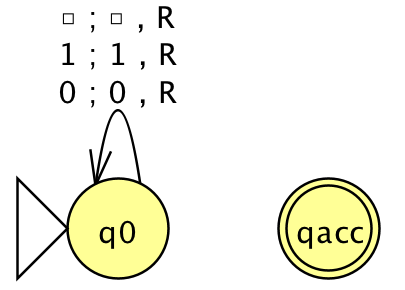
\includegraphics[width=1.5in]{../../resources/machines/Lect22TM1.png} ,  \varepsilon  \rangle$
    and  $M'$ is a Turing machine that computes like $M$ except, if the computation ever were to go to a  reject state,
    $M'$ loops instead.
    
    \vfill

    $F( \langle 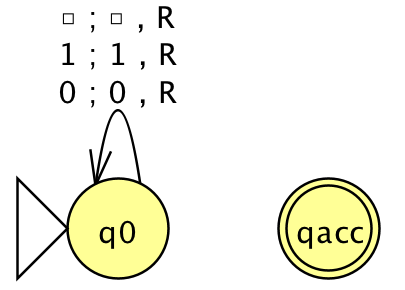
\includegraphics[width=1.5in]{../../resources/machines/Lect22TM1.png} ,  001  \rangle)$ =

    \vfill

    $F( \langle 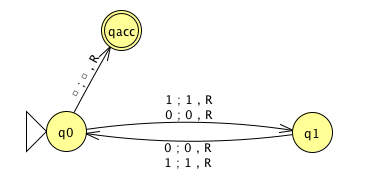
\includegraphics[width=2.5in]{../../resources/machines/Lect22TM2.png} ,  1  \rangle)$ =

    \vfill
    
    \newpage
    To use this function  to prove that $A_{TM} \leq_m HALT_{TM}$, we need  two claims:

    
    Claim (1): $F$ is computable \phantom{\hspace{2in}}
    
    \vfill

    Claim (2): for every  $x$,  $x \in  A_{TM}$ iff $F(x) \in HALT_{TM}$.  
    
    \vfill
   
    
\newpage
True or False: $\overline{A_{TM}} \leq_m \overline{HALT_{TM}}$

\vfill

True or False: $HALT_{TM} \leq_m A_{TM}$.

\vfill

\newpage \vfill
\section*{Week9 wednesday}




Recall:  $A$ is  {\bf  mapping  reducible to} $B$, written $A \leq_m B$,  means there is a computable function 
$f : \Sigma^* \to \Sigma^*$ such that {\it for all} strings  $x$ in $\Sigma^*$, 
\[
x  \in  A \qquad \qquad \text{if and  only  if} \qquad \qquad f(x) \in B.
\]



{\bf Theorem} (Sipser 5.28): If $A \leq_m B$ and $B$ is recognizable, then $A$ is recognizable.

{\bf Proof}: 


\vfill


{\bf Corollary}: If  $A \leq_m B$ and $A$ is unrecognizable, then $B$ is unrecognizable.


\vfill



{\it Strategy}:  

(i) To prove that a  recognizable language $R$ is undecidable, prove that $A_{TM} \leq_m R$.


(ii) To prove that a co-recognizable language $U$ is undecidable, prove that $\overline{A_{TM}} \leq_m U$,
 i.e. that $A_{TM} \leq_m \overline{U}$.

\newpage

\[
E_{TM} = \{ \langle M \rangle \mid \text{$M$ is a Turing machine and $L(M) = \emptyset$} \}
\]

Example  string in  $E_{TM}$ is \underline{\phantom{\hspace{1.6in}}} .
Example  string not  in  $E_{TM}$ is \underline{\phantom{\hspace{1.6in}}} .

$E_{TM}$ is ~~decidable /  undecidable~~ and ~~recognizable /  unrecognizable~~.

$\overline{E_{TM}}$ is ~~decidable /  undecidable~~ and ~~recognizable /  unrecognizable~~.


{\bf Claim}: $\underline{\phantom{\hspace{1.6in}}}  \leq_m \overline{E_{TM}}$.

{\bf Proof}: Need computable function  $F: \Sigma^* \to \Sigma^*$  such that  $x \in A_{TM}$ iff $F(x)  \notin  E_{TM}$.
Define
\begin{quote}
$F =  ``$ On input $x$,
\begin{itemize}
\item[1.] Type-check whether  $x = \langle M, w \rangle$ for some TM $M$ and string $w$.   If so, move to step 2; if  not, output 
\item[2.] Construct the following machine $M'_x$:
\vspace{50pt}
\item[3.] Output $\langle M'_x \rangle$."
\end{itemize}
\end{quote}

Verifying correctness:
\begin{center}
\begin{tabular}{|c|c|}
\hline
Input string &  Output string \\
\hline
$\langle M, w \rangle$ where  $w \in L(M)$ & \phantom{\hspace{4in}} \\
& \\
$\langle M, w \rangle$ where $w \notin L(M)$ & \\
&\\
$x$ not encoding any pair of  TM and string   &  \\
\hline
\end{tabular}
\end{center}

\newpage
\[
EQ_{TM} = \{ \langle M, M' \rangle \mid \text{$M$ and $M'$ are both Turing machines and $L(M) =L(M')$} \}
\]

Example  string in  $EQ_{TM}$ is \underline{\phantom{\hspace{1.5in}}} .
Example  string not  in  $EQ_{TM}$ is \underline{\phantom{\hspace{1.5in}}} .

$EQ_{TM}$ is ~~decidable /  undecidable~~ and ~~recognizable /  unrecognizable~~.

$\overline{EQ_{TM}}$ is ~~decidable /  undecidable~~ and ~~recognizable /  unrecognizable~~.

To  prove, show that  $\underline{\phantom{\hspace{1.6in}}}  \leq_m EQ_{TM}$
and that $\underline{\phantom{\hspace{1.6in}}}  \leq_m \overline{EQ_{TM}}$.


\vfill

Verifying correctness:
\begin{center}
\begin{tabular}{|c|c|}
\hline
Input string &  Output string \\
\hline
$\langle M, w \rangle$ where  $M$ halts on $w$ & \phantom{\hspace{4in}} \\
& \\
$\langle M, w \rangle$ where $M$ loops on $w$ & \\
&\\
$x$ not encoding any pair of  TM and string   &  \\
\hline
\end{tabular}
\end{center}

\vfill

\newpage \vfill
\section*{Week9 friday}



In practice, computers (and Turing machines) don't have infinite tape, 
and we can't afford to wait unboundedly long for an answer.
``Decidable" isn't good enough - we want ``Efficiently decidable".

For a given algorithm working on a given input, how long do we need to wait for an answer? 
How does the running time depend on the input in the worst-case? average-case? 
We expect to have to spend more time on computations with larger inputs.


A language is {\bf recognizable} if \underline{\phantom{\hspace{4.5in}}}

A language is {\bf decidable} if \underline{\phantom{\hspace{4.7in}}}

A language is {\bf efficiently  decidable} if \underline{\phantom{\hspace{4in}}}

A function is {\bf computable} if \underline{\phantom{\hspace{4.7in}}}

A function is {\bf efficiently computable} if \underline{\phantom{\hspace{4in}}}\\

\vfill

Definition  (Sipser 7.1): For  $M$ a deterministic decider, its {\bf running time} is the function  $f: \mathbb{N} \to \mathbb{N}$
given  by
\[
f(n) =  \text{max number of  steps $M$ takes before halting, over all inputs  of length $n$}
\]

Definition (Sipser 7.7): For each function $t(n)$, the {\bf time complexity class}  $TIME(t(n))$, is defined  by
\[
TIME( t(n)) = \{ L \mid \text{$L$ is decidable by  a Turing machine with running time in  $O(t(n))$} \}
\]

An example of an element of  $TIME(  1  )$ is 

An example of an element of  $TIME(  n  )$ is 


Note: $TIME( 1) \subseteq TIME (n)  \subseteq TIME(n^2)$

\vfill

Definition (Sipser 7.12) : $P$ is the class of languages that  are decidable in polynomial time on 
a deterministic 1-tape  Turing  machine
\[
P  =  \bigcup_k TIME(n^k)
\]

{\it Compare to exponential time: brute-force search.}


Theorem (Sipser 7.8): Let $t(n)$ be a  function with  $t(n)  \geq n$.  Then every $t(n)$ time deterministic 
multitape Turing machine has an equivalent $O(t^2(n))$ time deterministic 1-tape Turing machine.



\newpage


Definition (Sipser  7.9): For $N$ a nodeterministic decider.  
The {\bf running time} of $N$ is the function $f: \mathbb{N} \to \mathbb{N}$ given  by
\[
f(n) =  \text{max number of  steps $N$ takes on  any branch before halting, over all inputs  of length $n$}
\]

Definition (Sipser 7.21): For each function $t(n)$, the {\bf nondeterministic time complexity class}  
$NTIME(t(n))$, is defined  by
\[
NTIME( t(n)) = \{ L \mid \text{$L$ is decidable by a nondeterministic Turing machine with running time in $O(t(n))$} \}
\]
\[
NP = \bigcup_k NTIME(n^k)
\]


{\bf True} or {\bf False}: $TIME(n^2) \subseteq NTIME(n^2)$

\vfill

{\bf True} or {\bf False}: $NTIME(n^2) \subseteq DTIME(n^2)$

\vfill

{\bf Examples in $P$ }

{\it Can't use nondeterminism; Can use multiple tapes; Often need to be “more clever” than naïve / brute force approach}
\[
    PATH = \{\langle G,s,t\rangle \mid \textrm{$G$ is digraph with $n$ nodes there is path from s to t}\}
\]
Use breadth first search to show in $P$
\[
    RELPRIME = \{ \langle x,y\rangle \mid \textrm{$x$ and $y$ are relatively prime integers}\}
\]
Use Euclidean Algorithm to show in $P$
\[
    L(G) = \{w \mid \textrm{$w$ is generated by $G$}\} 
\]
(where $G$ is a context-free grammar). Use dynamic programming to show in $P$.

\vfill
{\bf Examples in $NP$}

{\it ``Verifiable" i.e. NP, Can be decided by a nondeterministic TM in polynomial time,
best known deterministic solution may be brute-force, 
solution can be verified by a deterministic TM in polynomial time.}

\[
    HAMPATH = \{\langle G,s,t \rangle \mid \textrm{$G$ is digraph with $n$ nodes, there is path
from $s$ to $t$ that goes through every node exactly once}\}
\]
\[
    VERTEX-COVER = \{ \langle G,k\rangle \mid \textrm{$G$ is an undirected graph with $n$
nodes that has a $k$-node vertex cover}\}
\]
\[
    CLIQUE = \{ \langle G,k\rangle \mid \textrm{$G$ is an undirected graph with $n$ nodes that has a $k$-clique}\}
\]
\[
    SAT =\{ \langle X \rangle \mid \textrm{$X$ is a satisfiable Boolean formula with $n$ variables}\}
\]

\newpage \vfill
\section*{Week8 monday}



{\bf  Theorem}: $A_{TM}$  is  not  Turing-decidable.

{\bf  Proof}: Suppose {\bf towards a  contradiction}  that there  is a Turing machine  that decides $A_{TM}$.  
We call this presumed machine  $M_{ATM}$.

By  assumption, for every  Turing machine  $M$ and every  string $w$

\begin{itemize}
\item If $w \in L(M)$, then  the computation of $M_{ATM}$  on  $\langle M,w \rangle ~~ \underline{\phantom{\hspace{2.5in}}}$
\item If $w \notin L(M)$, then  the computation of $M_{ATM}$  on  $\langle M,w \rangle ~~ \underline{\phantom{\hspace{2.5in}}}$
\end{itemize}


Define  a {\bf new} Turing machine using  the high-level description:
\begin{quote}
$D =  $`` On  input $\langle M \rangle$, where  $M$  is  a Turing machine:
\begin{itemize}
\item[1.] Run  $M_{ATM}$ on  $\langle M, \langle M \rangle  \rangle$.
\item[2.] If $M_{ATM}$ accepts, reject; if  $M_{ATM}$ rejects, accept."
\end{itemize}
\end{quote}


Is $D$ a  Turing machine?

\vspace{50pt}

Is  $D$ a  decider? 

\vspace{50pt}

What is the result of the computation  of $D$  on  $\langle D \rangle$?

\vfill

\newpage

{\bf  Theorem} (Sipser Theorem 4.22): A  language is Turing-decidable if and only if both  it and its complement
are Turing-recognizable.

{\bf Proof, first direction:}  Suppose  language  $L$ is  Turing-decidable.   WTS  that both it and its complement 
are Turing-recognizable.

\vfill

{\bf Proof, second direction:}  Suppose  language  $L$ is  Turing-recognizable, and  so is  its complement.   WTS  that $L$
is Turing-decidable.
\vfill


Give an example of a {\bf decidable} set: 

\vspace{20pt}

Give an example of a {\bf recognizable undecidable} set: 

\vspace{20pt}

Give an example of an {\bf unrecognizable} set: 

\vspace{20pt}


\newpage

{\bf True} or {\bf False}: The class of Turing-decidable languages is closed under complementation?

\vfill
\vfill
\vfill
Definition: A language $L$ over an  alphabet $\Sigma$ is called {\bf co-recognizable} if its complement,  defined
as $\Sigma^* \setminus L  = \{ x  \in  \Sigma^* \mid x \notin  L \}$, is Turing-recognizable.


Notation: The complement  of a set $X$ is denoted with  a superscript $c$, $X^c$, or an overline,  $\overline{X}$.
 \vfill
\section*{Week8 wednesday}


{\bf Mapping reduction}

Motivation: Proving that $A_{TM}$ is undecidable was hard. How can we leverage that work? 
Can we relate the decidability / undecidability of one problem to another?

\begin{quote}
If problem $X$ is {\bf no harder than} problem $Y$

\ldots and if $Y$ is easy,

\ldots then $X$ must be easy too.
\end{quote}


\begin{quote}
    If problem $X$ is {\bf no harder than} problem $Y$
    
    \ldots and if $X$ is hard,
    
    \ldots then $Y$ must be hard too.
\end{quote}

``Problem $X$ is no harder than problem $Y$'' means 
``Can answer questions about membership in $X$ by converting them to questions about membership in $Y$''.



Definition:  $A$ is  {\bf  mapping  reducible to} $B$  means there is a computable function 
$f : \Sigma^* \to \Sigma^*$ such that {\it for all} strings  $x$ in $\Sigma^*$, 
\[
x  \in  A \qquad \qquad \text{if and  only  if} \qquad \qquad f(x) \in B.
\]
Notation:  when $A$  is mapping reducible to $B$, we write $A  \leq_m B$.

{\it Intuition:} $A \leq_m B$ means $A$ is no harder than $B$, i.e. that the level 
of difficulty of $A$ is less than or equal the level of difficulty of $B$.

\vfill

\newpage
{\bf Computable functions}

Definition: A function $f: \Sigma^* \to \Sigma^*$ is a {\bf computable function} means there is some Turing machine such that, 
for each $x$, on input $x$ the Turing machine halts with exactly $f(x)$ followed by all blanks on the tape

{\it Examples of computable functions}:

The function that maps a string to a string which is one character longer and 
whose value, when interpreted as a fixed-width binary representation of a
nonnegative integer is twice the value of the input string (when interpreted as 
a fixed-width binary representation of a non-negative integer)
\[
f_1: \Sigma^* \to \Sigma^* \qquad  f_1(x)  = x0
\]

To prove $f_1$ is computable function, we define a Turing machine computing it.

{\it High-level description}
\begin{quote}
    ``On input $w$
    
    1. Append $0$ to $w$.
    
    2. Halt.''
\end{quote}

{\it Implementation-level description}
\begin{quote}
    ``On input $w$
    
    1. Sweep read-write head to the right until find first blank cell.
    
    2. Write 0.
    
    3. Halt.''
\end{quote}

{\it Formal definition} $(\{q0, qacc, qrej\}, \{0,1\}, \{0,1,\textvisiblespace\},\delta, q0, qacc, qrej)$
where $\delta$ is specified by the state diagram: 


\newpage


The function that maps a string to the result of repeating the string twice.
\[
f_2: \Sigma^* \to \Sigma^* \qquad f_2( x )  =  xx
\]

\vfill

The function that maps strings that are not the codes of Turing machines to the empty 
string and that maps strings that code Turing machines to the code of the 
related Turing machine that acts like the Turing machine coded by the input, except
that if this Turing machine coded by the input tries to reject, the 
new machine will go into a loop.
\[
f_3: \Sigma^* \to \Sigma^*  \qquad f_3( x )  =   \begin{cases}  \varepsilon \qquad&\text{if $x$ is not the code of  a TM} \\
\langle (Q \cup \{q_{trap} \}, \Sigma, \Gamma, \delta', q_0, q_{acc}, q_{rej} ) \rangle \qquad&\text{if $x = \langle (Q, \Sigma, \Gamma, \delta, q_0, q_{acc}, q_{rej} )\rangle$}\end{cases}
\]
where $q_{trap} \notin Q$ and 
\[\delta'( (q,x) ) = \begin{cases}
(r,y,d) &\text{if $q \in Q$, $x \in \Gamma$, $\delta ((q,x)) = (r,y,d)$, and  $r \neq  q_{rej}$} \\
(q_{trap}, \textvisiblespace, R) & \text{otherwise}
\end{cases}
\]
\vfill

\newpage


The function that maps strings that are not the codes of CFGs to the empty 
string and that maps strings that code CFGs to the code of a PDA that recognizes
the language generated by the CFG.


\vfill

{\it Other examples?}
 \vfill
\section*{Week8 friday}



Recall definition:  $A$ is  {\bf  mapping  reducible to} $B$  means there is a computable function 
$f : \Sigma^* \to \Sigma^*$ such that {\it for all} strings  $x$ in $\Sigma^*$, 
\[
x  \in  A \qquad \qquad \text{if and  only  if} \qquad \qquad f(x) \in B.
\]
Notation:  when $A$  is mapping reducible to $B$, we write $A  \leq_m B$.

{\it Intuition:} $A \leq_m B$ means $A$ is no harder than $B$, i.e. that the level 
of difficulty of $A$ is less than or equal the level of difficulty of $B$.


{\it Example}: $A_{TM} \leq_m A_{TM}$ 

\vfill

{\it Example}: $A_{DFA} \leq_m \{ ww \mid  w \in \{0,1\}^* \}$ 

\vfill



{\it Example}: $\{ 0^i  1^j \mid i  \geq 0, j \geq 0 \} \leq_m A_{TM}$ 

\vfill

{\bf Theorem} (Sipser 5.22): If $A \leq_m B$ and $B$ is decidable, then $A$ is decidable.
    

{\bf Theorem} (Sipser 5.23): If $A \leq_m B$ and $A$ is undecidable, then $B$ is undecidable.
    

\newpage

    {\bf Halting problem}
    \[
    HALT_{TM} = \{ \langle M, w \rangle \mid \text{$M$ is a  Turing machine, $w$ is  a string, and $M$ halts on $w$} \}
    \]
    
    Define $F: \Sigma^* \to \Sigma^*$ by
    \[
    F(x) =  \begin{cases}
    const_{out} \qquad &\text{if  $x \neq \langle M,w \rangle$ for any Turing machine  $M$ and string  $w$ over the alphabet of $M$} \\
    \langle M', w \rangle \qquad &  \text{if $x = \langle M, w \rangle$ for some Turing machine  $M$ and string $w$ over the alphabet of $M$.}
    \end{cases}
    \]
    where $const_{out}  =  \langle  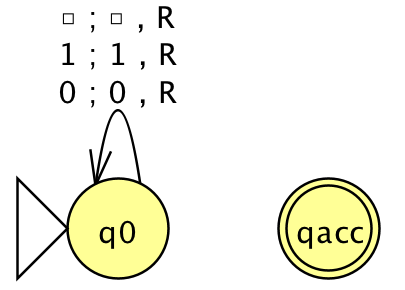
\includegraphics[width=1.5in]{../../resources/machines/Lect22TM1.png} ,  \varepsilon  \rangle$
    and  $M'$ is a Turing machine that computes like $M$ except, if the computation ever were to go to a  reject state,
    $M'$ loops instead.
    
    \vfill

    $F( \langle 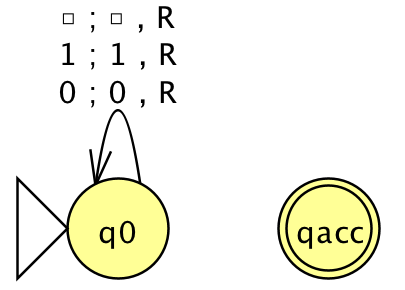
\includegraphics[width=1.5in]{../../resources/machines/Lect22TM1.png} ,  001  \rangle)$ =

    \vfill

    $F( \langle 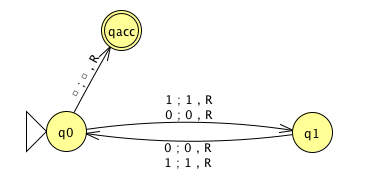
\includegraphics[width=2.5in]{../../resources/machines/Lect22TM2.png} ,  1  \rangle)$ =

    \vfill
    
    \newpage
    To use this function  to prove that $A_{TM} \leq_m HALT_{TM}$, we need  two claims:

    
    Claim (1): $F$ is computable \phantom{\hspace{2in}}
    
    \vfill

    Claim (2): for every  $x$,  $x \in  A_{TM}$ iff $F(x) \in HALT_{TM}$.  
    
    \vfill
     \vfill
\section*{Week6 monday}


For Turing machine $M= (Q, \Sigma, \Gamma, \delta, q_0, q_{accept}, q_{reject})$ 
the {\bf computation} of $M$ on a string $w$ over $\Sigma$  is:

\vspace{-20pt}

\begin{itemize}
\setlength{\itemsep}{0pt}
\item Read/write head starts at leftmost position on tape. 
\item Input string is written on $|w|$-many leftmost cells of tape, 
rest of  the tape cells have  the blank symbol. {\bf Tape alphabet} 
is $\Gamma$ with $\textvisiblespace\in \Gamma$ and $\Sigma \subseteq \Gamma$.
The blank symbol $\textvisiblespace \notin \Sigma$.
\item Given current state of machine and current symbol being read at the tape head, 
the machine transitions to next state, writes a symbol to the current position  of the 
tape  head (overwriting existing symbol), and moves the tape head L or R (if possible). 
Formally, {\bf transition function}  is 
\[
  \delta: Q\times \Gamma \to Q \times \Gamma \times \{L, R\}
\]
\item Computation ends if and when machine enters either the accept or the reject state.
This is called {\bf halting}.
Note: $q_{accept} \neq q_{reject}$.
\end{itemize}

The {\bf language recognized by the  Turing machine} $M$,  is  
\[
  \{ w \in \Sigma^* \mid \textrm{computation of $M$ on $w$ halts after entering the accept state}\} = \{ w \in \Sigma^* \mid w \textrm{ is accepted by } M\}
\]
  
To define a Turing machine, we could give a 
\begin{itemize}
\item {\bf Formal definition}, namely the $7$-tuple of parameters including set of states, 
input alphabet, tape alphabet, transition function, start state, accept state, and reject state; or,
\item {\bf Implementation-level definition}: English prose that describes the Turing machine head 
movements relative to contents of tape, and conditions for accepting / rejecting based on those contents.
\end{itemize}

Conventions for drawing state diagrams of Turing machines: (1) omit the reject state from the diagram (unless 
it's the  start state), (2) any missing transitions in the state diagram have value $(q_{reject}, ~\textvisiblespace~ , R)$.


\newpage
{\it Sipser Figure  3.10}

\begin{multicols}{2}
\vspace{-20pt}
\begin{center}
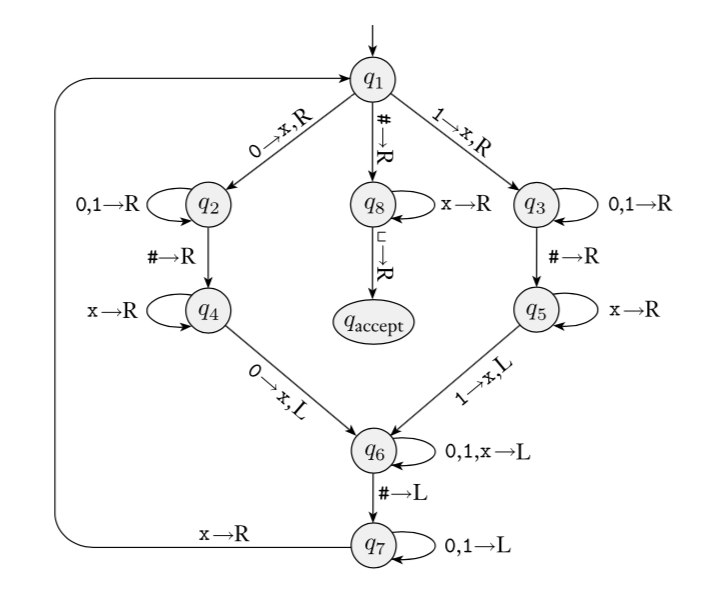
\includegraphics[width=4in]{../../resources/machines/Lect13TM3.png}
\end{center}

Implementation level description of this machine:
\begin{quote}
Zig-zag across tape to corresponding positions on either side of $\#$ to check whether the 
characters in these positions agree. If they do not, or if there is no $\#$, reject. If they 
do, cross them off.

Once all symbols to the left of the $\#$ are crossed off, check for any un-crossed-off symbols 
to the right of $\#$; if there are any, reject; if there aren't, accept.
\end{quote}

\columnbreak

Computation on  input  string  $01\#01$

\begin{tabular}{|c|c|c|c|c|c|c|}
\hline
\multicolumn{1}{|c}{$q_1 \downarrow$} &  \multicolumn{6}{c|}{\phantom{A}}\\
\hline
$0$ & $1$  & $\#$  & $0$ & $1$ & $\textvisiblespace $& $\textvisiblespace $\\
\hline
  \multicolumn{7}{|c|}{\phantom{A}}\\
  \hline
  \phantom{AA} & \phantom{AA}& \phantom{AA}& \phantom{AA}& \phantom{AA}& \phantom{AA}& \phantom{AA} \\
  \hline
  \multicolumn{7}{|c|}{\phantom{A}}\\
  \hline
  \phantom{AA} & \phantom{AA}& \phantom{AA}& \phantom{AA}& \phantom{AA}& \phantom{AA}& \phantom{AA} \\
  \hline
  \multicolumn{7}{|c|}{\phantom{A}}\\
  \hline
  \phantom{AA} & \phantom{AA}& \phantom{AA}& \phantom{AA}& \phantom{AA}& \phantom{AA}& \phantom{AA} \\
  \hline
  \multicolumn{7}{|c|}{\phantom{A}}\\
  \hline
  \phantom{AA} & \phantom{AA}& \phantom{AA}& \phantom{AA}& \phantom{AA}& \phantom{AA}& \phantom{AA} \\
  \hline
  \multicolumn{7}{|c|}{\phantom{A}}\\
  \hline
  \phantom{AA} & \phantom{AA}& \phantom{AA}& \phantom{AA}& \phantom{AA}& \phantom{AA}& \phantom{AA} \\
  \hline
  \multicolumn{7}{|c|}{\phantom{A}}\\
  \hline
  \phantom{AA} & \phantom{AA}& \phantom{AA}& \phantom{AA}& \phantom{AA}& \phantom{AA}& \phantom{AA} \\
  \hline
  \multicolumn{7}{|c|}{\phantom{A}}\\
  \hline
  \phantom{AA} & \phantom{AA}& \phantom{AA}& \phantom{AA}& \phantom{AA}& \phantom{AA}& \phantom{AA} \\
  \hline
  \multicolumn{7}{|c|}{\phantom{A}}\\
  \hline
  \phantom{AA} & \phantom{AA}& \phantom{AA}& \phantom{AA}& \phantom{AA}& \phantom{AA}& \phantom{AA} \\
  \hline
  \multicolumn{7}{|c|}{\phantom{A}}\\
  \hline
  \phantom{AA} & \phantom{AA}& \phantom{AA}& \phantom{AA}& \phantom{AA}& \phantom{AA}& \phantom{AA} \\
  \hline
  \multicolumn{7}{|c|}{\phantom{A}}\\
  \hline
  \phantom{AA} & \phantom{AA}& \phantom{AA}& \phantom{AA}& \phantom{AA}& \phantom{AA}& \phantom{AA} \\
  \hline
  \multicolumn{7}{|c|}{\phantom{A}}\\
  \hline
  \phantom{AA} & \phantom{AA}& \phantom{AA}& \phantom{AA}& \phantom{AA}& \phantom{AA}& \phantom{AA} \\
  \hline
  \multicolumn{7}{|c|}{\phantom{A}}\\
  \hline
  \phantom{AA} & \phantom{AA}& \phantom{AA}& \phantom{AA}& \phantom{AA}& \phantom{AA}& \phantom{AA} \\
  \hline
  \multicolumn{7}{|c|}{\phantom{A}}\\
  \hline
  \phantom{AA} & \phantom{AA}& \phantom{AA}& \phantom{AA}& \phantom{AA}& \phantom{AA}& \phantom{AA} \\
  \hline
  \multicolumn{7}{|c|}{\phantom{A}}\\
  \hline
  \phantom{AA} & \phantom{AA}& \phantom{AA}& \phantom{AA}& \phantom{AA}& \phantom{AA}& \phantom{AA} \\
  \hline
  \multicolumn{7}{|c|}{\phantom{A}}\\
  \hline
  \phantom{AA} & \phantom{AA}& \phantom{AA}& \phantom{AA}& \phantom{AA}& \phantom{AA}& \phantom{AA} \\
  \hline
  \multicolumn{7}{|c|}{\phantom{A}}\\
  \hline
  \phantom{AA} & \phantom{AA}& \phantom{AA}& \phantom{AA}& \phantom{AA}& \phantom{AA}& \phantom{AA} \\
  \hline
  \multicolumn{7}{|c|}{\phantom{A}}\\
  \hline
  \phantom{AA} & \phantom{AA}& \phantom{AA}& \phantom{AA}& \phantom{AA}& \phantom{AA}& \phantom{AA} \\
  \hline
  \multicolumn{7}{|c|}{\phantom{A}}\\
  \hline
  \phantom{AA} & \phantom{AA}& \phantom{AA}& \phantom{AA}& \phantom{AA}& \phantom{AA}& \phantom{AA} \\
  \hline
  \end{tabular}
\end{multicols}

The language recognized by this machine is
\[
  \{ w \# w \mid w \in \{0,1\}^* \}
\]

\newpage

  A language $L$ is {\bf recognized by} a Turing machine $M$ means

  \vspace{20pt}

  A Turing  machine  $M$ {\bf  recognizes} a language $L$ if means

  \vspace{20pt}
  
  A Turing machine $M$ is a {\bf decider}  means

  \vspace{20pt}
  
  A language  $L$ is {\bf decided by} a Turing  machine  $M$  means

  \vspace{20pt}
  
  A  Turing machine $M$ {\bf decides} a language $L$ means

  \vspace{20pt}
  
  
  Fix $\Sigma = \{0,1\}$, $\Gamma = \{ 0, 1, \textvisiblespace\}$ for the Turing machines with  the following state diagrams:
  
  \vspace{-35pt}
  
  
  \begin{center}
  \begin{tabular}{|c|c|}
  \hline
  \hspace{0.8in}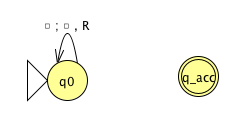
\includegraphics[width=2in]{../../resources/machines/Lect14TM1.png} \phantom{\hspace{0.8in}}&\hspace{0.8in} 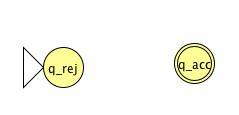
\includegraphics[width=2in]{../../resources/machines/Lect14TM2.png} \phantom{\hspace{0.8in}}\\
  Implementation  level description:  \phantom{\hspace{1in}} &Implementation  level description:  \phantom{\hspace{1in}} \\
  &\\
  &\\
  &\\
  Example of string accepted: \phantom{\hspace{1.5in}}& Example of string accepted: \phantom{\hspace{1.5in}}\\
  Example of string rejected: \phantom{\hspace{1.5in}}& Example of string  rejected: \phantom{\hspace{1.5in}}\\
  &\\
  Decider? Yes~~~/ ~~~No
  &Decider? Yes~~~/ ~~~No\\
  & \\
  \hline
  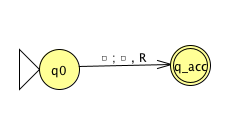
\includegraphics[width=2in]{../../resources/machines/Lect14TM3.png} & 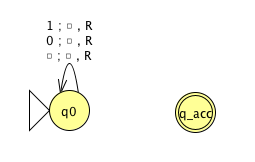
\includegraphics[width=2in]{../../resources/machines/Lect14TM4.png} \\
  Implementation  level description:  \phantom{\hspace{1in}} &Implementation  level description:  \phantom{\hspace{1in}} \\
  &\\
  &\\
  &\\
  Example of string accepted: \phantom{\hspace{1.5in}}& Example of string accepted: \phantom{\hspace{1.5in}}\\
  Example of string rejected: \phantom{\hspace{1.5in}}& Example of string  rejected: \phantom{\hspace{1.5in}}\\
  &\\
  Decider? Yes~~~/ ~~~No
  &Decider? Yes~~~/ ~~~No\\
  & \\
  
  \hline
  \end{tabular}
  \end{center} \vfill
\section*{Week6 wednesday}


Two models of computation are called {\bf equally expressive} when 
every language recognizable with the first model is recognizable with the second, and vice versa.

True / False: NFAs and PDAs are equally expressive.

True / False: Regular expressions and CFGs are equally expressive.


\begin{center}
{\large \it  Some examples of models that are {\bf equally expressive} with deterministic Turing machines: }
\end{center}

\fbox{ {\bf May-stay}  machines }
The May-stay machine model is the same as the usual Turing machine model,  except that
on each transition, the tape head may move L, move R, or Stay. 

Formally: $(Q, \Sigma, \Gamma, \delta, q_0, q_{accept}, q_{reject})$ where 
\[
  \delta: Q \times \Gamma \to Q \times \Gamma \times \{L, R, S\}
\]

{\bf Claim}: Turing machines and May-stay machines are equally expressive. {\it To prove \ldots}

To translate a standard TM to a may-stay machine: 

\vspace{100pt}




To translate one  of the  may-stay machines to standard TM:
any time TM would Stay, move right  then  left.


Formally: suppose $M_S =  (Q, \Sigma, \Gamma, \delta, q_0, q_{acc}, q_{rej})$
has $\delta: Q \times \Gamma \to Q \times \Gamma \times \{L, R, S\}$. Define
the Turing-machine
\[
  M_{new} =  (\phantom{\hspace{2.5in}})
\]

\vfill

\newpage

\phantom{$M_{new}$ construction here \vspace{400pt}}
\vfill


\fbox{ {\bf Multitape Turing machine}} A multitape Turing macihne with $k$ tapes
can be formally representated as 
$(Q, \Sigma,  \Gamma, \delta, q_0, q_{acc}, q_{rej})$ 
where $Q$ is the finite set of  states,
$\Sigma$ is the  input alphabet with  $\textvisiblespace \notin \Sigma$,
$\Gamma$  is the  tape alphabet with $\Sigma \subsetneq \Gamma$ ,
$\delta: Q\times \Gamma^k\to Q \times \Gamma^k \times \{L,R\}^k$ 
(where $k$ is  the number of  states)


If $M$ is a standard  TM, it is a $1$-tape machine.


To translate a $k$-tape machine  to  a standard TM:
Use a  new symbol to separate the contents of each tape
and keep track of location of  head with  special version of each
tape symbol. {\tiny Sipser Theorem 3.13} 

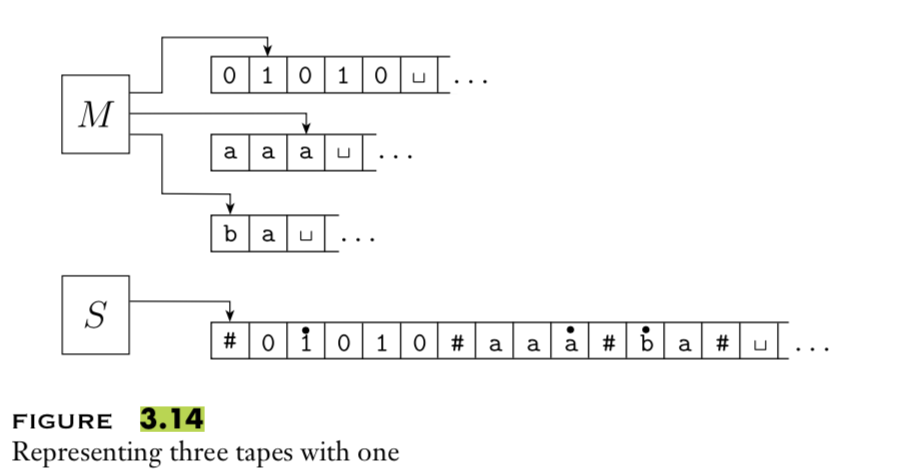
\includegraphics[width=2.5in]{../../resources/images/Figure314.png}


{\it Extra practice:} \fbox{ {\bf  Wikipedia Turing machine} }
Define a machine $(Q, \Gamma, b, \Sigma,  q_0, F, \delta)$
where $Q$ is the finite set  of  states
$\Gamma$  is the tape alphabet,
$b \in \Gamma$ is the blank symbol, 
$\Sigma \subsetneq \Gamma$ is the  input alphabet, 
$q_0 \in  Q$ is the start state, 
$F \subseteq Q$ is the set of accept states, 
$\delta: (Q \setminus F)  \times  \Gamma \not\to Q \times  \Gamma  \times \{L, R\}$
 is a partial transition function
If computation enters a state  in $F$, it  accepts 
If computation enters a configuration where
 $\delta$ is not defined, it  rejects . {\tiny Hopcroft and  Ullman, cited by  Wikipedia} 

\newpage
\fbox{ {\bf Enumerators} } Enumerators give a different
model of computation where a language is {\bf produced, one string at a time},
rather than recognized by accepting (or not) individual strings.

Each enumerator machine has finite state control, unlimited work tape, and a printer. The computation proceeds
according to transition function; at any point machine may ``send'' a string to the printer.
\[
E  = (Q, \Sigma, \Gamma, \delta, q_0, q_{print})  
\]
$Q$ is the finite set of states, $\Sigma$ is  the output alphabet, $\Gamma$ is the 
tape alphabet ($\Sigma  \subsetneq\Gamma, 
\textvisiblespace \in \Gamma \setminus \Sigma$), 
\[
\delta:  Q  \times  \Gamma \times \Gamma \to  Q \times  \Gamma \times  \Gamma \times \{L, R\} \times  \{L, R\}
\]
where in state $q$, when the working tape is scanning character $x$ and the printer tape is scanning character $y$,
$\delta( (q,x,y) ) = (q', x', y', d_w, d_p)$ means transition to control state $q'$, write $x'$ on 
the working tape, write $y'$ on the printer tape, move in direction $d_w$ on the working tape, and move in direction 
$d_p$ on the printer tape. The computation starts in $q_0$ and each time the computation enters $q_{print}$
the string from the leftmost edge of the printer tape to the first blank cell is considered to be printed.

The language  {\bf  enumerated} by  $E$, $L(E)$, is $\{ w \in \Sigma^* \mid \text{$E$ eventually, at finite  time, 
prints $w$} \}$.


\begin{center}
\begin{tabular}{cc}
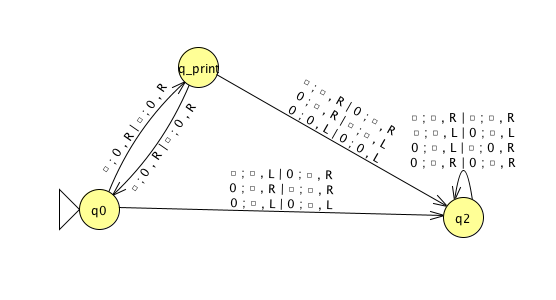
\includegraphics[width=3.5in]{../../resources/machines/Lec15enumerator.png}  & 
\begin{tabular}{|c|c|c|c|c|c|c|}
\hline
\multicolumn{1}{|c}{$q0$} &  \multicolumn{6}{c|}{\phantom{A}}\\
\hline
$\textvisiblespace ~*$& $\textvisiblespace$  & $\textvisiblespace$ & $\textvisiblespace$& $\textvisiblespace$& $\textvisiblespace$&  $\textvisiblespace$\\
\hline
$\textvisiblespace  ~*$& $\textvisiblespace$  & $\textvisiblespace$ & $\textvisiblespace$& $\textvisiblespace$& $\textvisiblespace$&  $\textvisiblespace$\\
\hline\hline
\multicolumn{7}{|c|}{\phantom{A}}\\
\hline
\phantom{AA} & \phantom{AA}& \phantom{AA}& \phantom{AA}& \phantom{AA}& \phantom{AA}& \phantom{AA} \\
\hline
\phantom{AA} & \phantom{AA}& \phantom{AA}& \phantom{AA}& \phantom{AA}& \phantom{AA}& \phantom{AA} \\
\hline
\hline
\multicolumn{7}{|c|}{\phantom{A}}\\
\hline
\phantom{AA} & \phantom{AA}& \phantom{AA}& \phantom{AA}& \phantom{AA}& \phantom{AA}& \phantom{AA} \\
\hline
\phantom{AA} & \phantom{AA}& \phantom{AA}& \phantom{AA}& \phantom{AA}& \phantom{AA}& \phantom{AA} \\
\hline
\hline
\multicolumn{7}{|c|}{\phantom{A}}\\
\hline
\phantom{AA} & \phantom{AA}& \phantom{AA}& \phantom{AA}& \phantom{AA}& \phantom{AA}& \phantom{AA} \\
\hline
\phantom{AA} & \phantom{AA}& \phantom{AA}& \phantom{AA}& \phantom{AA}& \phantom{AA}& \phantom{AA} \\
\hline
\hline
\multicolumn{7}{|c|}{\phantom{A}}\\
\hline
\phantom{AA} & \phantom{AA}& \phantom{AA}& \phantom{AA}& \phantom{AA}& \phantom{AA}& \phantom{AA} \\
\hline
\phantom{AA} & \phantom{AA}& \phantom{AA}& \phantom{AA}& \phantom{AA}& \phantom{AA}& \phantom{AA} \\
\hline
\end{tabular}
\end{tabular}
\end{center}


\vfill 

{\bf Theorem 3.21} A language is Turing-recognizable iff some enumerator enumerates it.
{\it Proof next time \ldots } \vfill
\section*{Week6 friday}



To define a Turing machine, we could give a 
\begin{itemize}
\item {\bf Formal definition}: the $7$-tuple of parameters including set of states, 
input alphabet, tape alphabet, transition function, start state, accept state, and reject state; or,
\item {\bf Implementation-level definition}: English prose that describes the Turing machine head 
movements relative to contents of tape, and conditions for accepting / rejecting based on those contents.
\item {\bf High-level description}: description of algorithm (precise sequence of instructions), 
without implementation details of machine. As part of this description, can ``call" and run 
another TM as a subroutine.
\end{itemize}


{\bf Theorem 3.21} A language is Turing-recognizable iff some enumerator enumerates it.

{\bf Proof}:

Assume $L$ is enumerated by some enumerator, $E$, so $L = L(E)$.
We'll use $E$ in a subroutine
within a high-level description of a new Turing machine that we will build to recognize $L$.

{\bf Goal}: build Turing machine $M_E$ with $L(M_E) = L(E)$.

Define $M_E$ as follows: $M_E = $ ``On input $w$,
\begin{enumerate}
\item Run $E$. For each string $x$ printed by $E$.
\item \qquad Check if $x = w$. If so, accept (and halt); otherwise, continue."
\end{enumerate}


\vfill 



Assume $L$ is Turing-recognizable and there 
is a Turing  machine  $M$ with  $L = L(M)$. We'll use $M$ in a subroutine
within a high-level description of an enumerator that we will build to enumerate $L$.

{\bf Goal}: build enumerator $E_M$ with $L(E_M) = L(M)$.

{\bf Idea}: check each string in turn to see if it is in $L$.

{\it How?} Run computation of $M$ on each string.  {\it But}: need to be careful 
about computations that don't halt.

{\it Recall} String order for $\Sigma = \{0,1\}$: $s_1 = \varepsilon$, $s_2 = 0$, $s_3 = 1$, $s_4 = 00$, $s_5 = 01$, $s_6  = 10$, 
$s_7  =  11$, $s_8 = 000$, \ldots

Define $E_M$ as follows: $E_{M} = $ `` {\it ignore any input.} Repeat the following for $i=1, 2, 3, \ldots$
\begin{enumerate}
  \item Run the computations of $M$ on $s_1$, $s_2$, \ldots, $s_i$ for (at most) $i$ steps each
  \item For each of these $i$ computations that accept during the (at most) $i$ steps, print
  out the accepted string."
\end{enumerate}

\newpage

{\bf Nondeterministic Turing machine}

At any point in the computation, the nondeterministic machine may proceed according to 
several possibilities: $(Q, \Sigma, \Gamma, \delta, q_0, q_{acc}, q_{rej})$ where 
\[
\delta: Q \times \Gamma \to \mathcal{P}(Q \times \Gamma \times \{L, R\})  
\]
The computation of a nondeterministic Turing machine is a tree with branching
when the next step of the computation has multiple possibilities. A nondeterministic
Turing machine accepts a string exactly when some branch of the computation tree 
enters the accept state.

Given a nondeterministic machine, we can use a $3$-tape Turing machine to 
simulate it by doing a breadth-first search of computation tree: one tape 
is ``read-only'' input tape, one tape simulates the tape of the nondeterministic
computation, and one tape tracks nondeterministic branching. {\tiny Sipser page 178} 

\vfill
Two models of computation are called {\bf equally expressive} when 
every language recognizable with the first model is recognizable with the second, and vice versa.

{\bf  Church-Turing Thesis} (Sipser p. 183): The informal notion of algorithm is formalized completely  and correctly by the 
formal definition of a  Turing machine. In other words: all reasonably expressive models of 
computation are equally expressive with the standard Turing machine.

\vfill

\newpage

{\bf Claim}: If two languages  (over a fixed alphabet  $\Sigma$) are Turing-recognizable, then  their union  is  as well.

{\bf Proof using Turing machines}:

\vfill

{\bf Proof using nondeterministic Turing machines}: 

\vfill  

{\bf  Proof using enumerators}:

\vfill

 \vfill
\section*{Week7 monday}



\begin{center}
    \begin{tabular}{|l|l|l|l|}
    \hline
    & Suppose $M$ is  a TM & Suppose $D$ is  a TM & Suppose $E$ is  an
    enumerator  \\
    &that  recognizes $L$  &that  decides $L$  &that enumerates $L$ \\
    \hline
    If string $w$ is in  $L$ then  \ldots  &&& \\
    &&&\\
    &&&\\
    If string $w$ is not in  $L$ then  \ldots  && &\\
    &&&\\
    &&&\\
    \hline
    \end{tabular}
\end{center}
    
    {\bf Describing  Turing machines} (Sipser p. 185)
    
    The Church-Turing thesis posits that each algorithm can be implemented by some Turing machine

    High-level descriptions of  Turing machine algorithms are written as indented text within quotation marks.   

    Stages of the algorithm are typically numbered consecutively.

    The first line specifies the input to the machine, which must be a string.
    This string may be the encoding of some object or  list of  objects.  
    
    {\bf Notation:} $\langle O \rangle$ is the string that encodes the object $O$.
    $\langle O_1, \ldots, O_n \rangle$ is the string that encodes the list of objects $O_1, \ldots, O_n$.
    
    {\bf Assumption}: There are Turing  machines that can be called as subroutines
    to decode the string representations of common objects and  interact with these objects as intended
    (data structures).
    
    \newpage    
    For example, since there are algorithms to answer each of the following questions,
    by Church-Turing thesis, there is a Turing machine that accepts exactly those strings for which the 
    answer to the question is ``yes''
    \begin{itemize}
        \item Does a string over $\{0,1\}$ have even length?

        \vfill

        \item Does a string over $\{0,1\}$ encode a string of ASCII characters?\footnote{An introduction to ASCII 
        is available on the w3 tutorial \href{https://www.w3schools.com/charsets/ref_html_ascii.asp}{here}.}

        \vfill

        \item Does a DFA have a specific number of states?

        \vfill

        \item Do two NFAs have any state names in common?

        \vfill

        \item Do two CFGs have the same start variable?

        \vfill

      \end{itemize}

\newpage

A {\bf computational problem} is decidable iff language encoding its positive problem instances
is decidable.

The computational problem ``Does a specific DFA accept a given string?'' is encoded by the language
\begin{align*}
  &\{ \textrm{representations of DFAs $M$ and strings $w$ such that $w \in L(M)$}\}  \\
  =& \{ \langle M, w \rangle \mid M \textrm{ is a DFA}, w \textrm{ is a string}, w \in L(M) \}
\end{align*}

The computational problem ``Is the language generated by a CFG empty?'' is encoded by the language
\begin{align*}
  &\{ \textrm{representations of CFGs $G$  such that $L(G) = \emptyset$}\}  \\
  =& \{ \langle G \rangle \mid G \textrm{ is a CFG},  L(G) = \emptyset \}
\end{align*}



The computational problem ``Is the given Turing machine a decider?'' is encoded by the language
\begin{align*}
  &\{ \textrm{representations of TMs $M$  such that $M$ halts on every input}\}  \\
  =& \{ \langle M \rangle \mid M \textrm{ is a TM and for each string } w, \textrm{$M$ halts on $w$} \}
\end{align*}


{\it Note: writing down the language encoding a computational problem is only the first step in 
determining if it's recognizable, decidable, or \ldots }


{\bf Some classes of computational problems help us understand the differences between the machine models we've been studying:}

\vspace{-20pt}

    \begin{center}
    \begin{tabular}{|lcl|}
    \hline
    \multicolumn{3}{|l|}{{\bf  Acceptance problem} } \\
    & & \\
    \ldots for DFA & $A_{DFA}$ & $\{ \langle B,w \rangle \mid  \text{$B$ is a  DFA that accepts input 
    string $w$}\}$ \\
    \ldots for NFA & $A_{NFA}$ & $\{ \langle B,w \rangle \mid  \text{$B$ is a  NFA that accepts input 
    string $w$}\}$ \\
    \ldots for regular expressions & $A_{REX}$ & $\{ \langle R,w \rangle \mid  \text{$R$ is a  regular
    expression that generates input string $w$}\}$ \\
    \ldots for CFG & $A_{CFG}$ & $\{ \langle G,w \rangle \mid  \text{$G$ is a context-free grammar 
    that generates input string $w$}\}$ \\
    \ldots for PDA & $A_{PDA}$ & $\{ \langle B,w \rangle \mid  \text{$B$ is a PDA that accepts input string $w$}\}$ \\
    & & \\
    & & \\
    \hline
    \multicolumn{3}{|l|}{{\bf Language emptiness  testing} } \\
    & & \\
    \ldots for DFA & $E_{DFA}$ & $\{ \langle A \rangle \mid  \text{$A$ is a  DFA and  $L(A) = \emptyset$\}}$ \\
    \ldots for NFA & $E_{NFA}$ & $\{ \langle A\rangle \mid  \text{$A$ is a NFA and  $L(A) = \emptyset$\}}$ \\
    \ldots for regular expressions & $E_{REX}$ & $\{ \langle R \rangle \mid  \text{$R$ is a  regular
    expression and  $L(R) = \emptyset$\}}$ \\
    \ldots for CFG & $E_{CFG}$ & $\{ \langle G \rangle \mid  \text{$G$ is a context-free grammar 
    and  $L(G) = \emptyset$\}}$ \\
    \ldots for PDA & $E_{PDA}$ & $\{ \langle A \rangle \mid  \text{$A$ is a PDA and  $L(A) = \emptyset$\}}$ \\
    & & \\
    & & \\
    \hline
    \multicolumn{3}{|l|}{{\bf Language equality testing} } \\
    & & \\
    \ldots for DFA & $EQ_{DFA}$ & $\{ \langle A, B \rangle \mid  \text{$A$ and $B$ are DFAs and  $L(A) =L(B)$\}}$\\
    \ldots for NFA & $EQ_{NFA}$ & $\{ \langle A, B \rangle \mid  \text{$A$ and $B$ are NFAs and  $L(A) =L(B)$\}}$\\
    \ldots for regular expressions & $EQ_{REX}$ & $\{ \langle R, R' \rangle \mid  \text{$R$ and $R'$ are regular
    expressions and  $L(R) =L(R')$\}}$\\
    \ldots for CFG & $EQ_{CFG}$ & $\{ \langle G, G' \rangle \mid  \text{$G$ and $G'$ are CFGs and  $L(G) =L(G')$\}}$ \\
    \ldots for PDA & $EQ_{PDA}$ & $\{ \langle A, B \rangle \mid  \text{$A$ and $B$ are PDAs and  $L(A) =L(B)$\}}$ \\
    \hline
    Sipser Section 4.1 &&\\
    \hline
    \end{tabular}
    \end{center}
    
    
    
    \newpage
    
    \begin{center}
    \begin{tabular}{|c|c|c|}
    \hline
    $M_1$  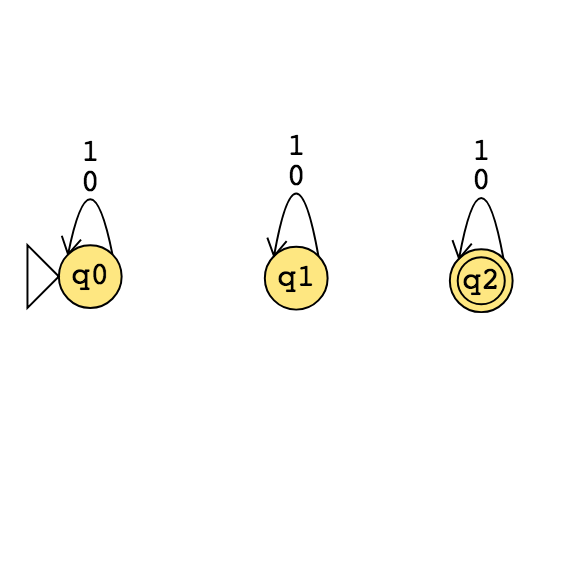
\includegraphics[width=2in]{../../resources/machines/Lect17DFA1.png} &  
    $M_2$ 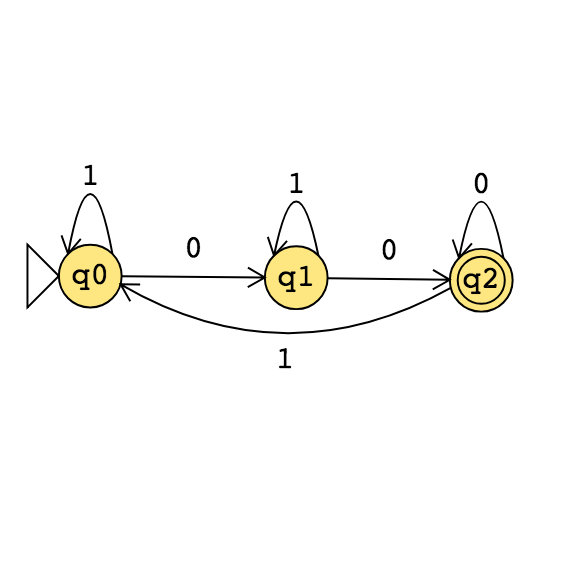
\includegraphics[width=2in]{../../resources/machines/Lect17DFA2.png} &  
    $M_3$ 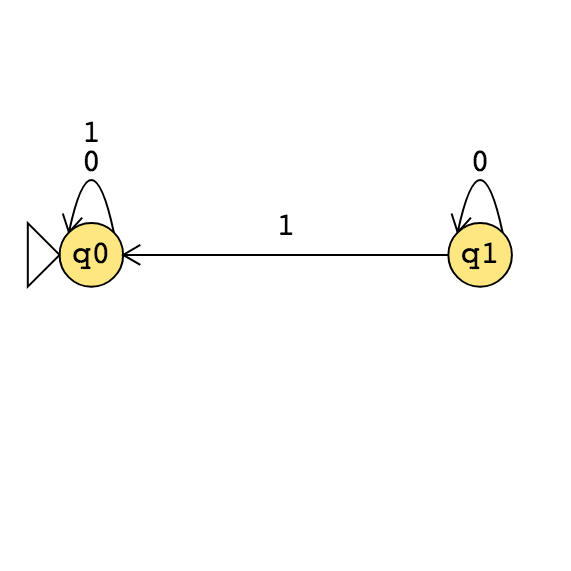
\includegraphics[width=2in]{../../resources/machines/Lect17DFA3.png} \\ 
    && \\
    && \\
    && \\
    && \\
    \hline
    \end{tabular}
    \end{center}
    
    Example strings in $A_{DFA}$
    
    \vfill
    
    Example strings in  $E_{DFA}$
    
    \vfill
    
    Example strings in  $EQ_{DFA}$
    
    \vfill

    Food for thought: which of the following computational problems are decidable: $A_{DFA}$?, $E_{DFA}$?, $EQ_{DFA}$?  \vfill
\section*{Week7 wednesday}


Deciding a computational problem means building / defining a Turing 
machine that recognizes the language encoding the computational problem, and that 
is a decider.

\begin{center}
  \begin{tabular}{|lcl|}
  \hline
  \multicolumn{3}{|l|}{{\bf  Acceptance problem} } \\
  for \ldots  & $A_{\ldots}$ & $\{ \langle B,w \rangle \mid  \text{$B$ is a \ldots that accepts input 
  string $w$}\}$ \\
  \hline
  \multicolumn{3}{|l|}{{\bf Language emptiness  testing} } \\
   for \ldots & $E_{\ldots}$ & $\{ \langle A \rangle \mid  \text{$A$ is a \ldots and  $L(A) = \emptyset$\}}$ \\
  \hline
  \multicolumn{3}{|l|}{{\bf Language equality testing} } \\
   for \ldots & $EQ_{\ldots}$ & $\{ \langle A, B \rangle \mid  \text{$A$ and $B$ are \ldots and  $L(A) =L(B)$\}}$\\
  \hline
  Sipser Section 4.1 &&\\
  \hline
  \end{tabular}
  \end{center}
  
  \begin{quote}
  $M_1 = $ ``On input $\langle M,w\rangle$, where $M$ is a DFA and $w$ is a string:
  \begin{enumerate}
  \setcounter{enumi}{-1}
  \item Type check encoding to check input is correct type.
  \item Simulate $M$ on input $w$ (by keeping track of states in $M$, transition function of $M$, etc.) 
  \item If the simulations ends in an accept state of $M$, accept. If it ends in a non-accept state of $M$, reject. "
  \end{enumerate}
  \end{quote}
  

What is $L(M_1)$? 

\vfill

Is $L(M_1)$ a decider?

\vfill

  
  \begin{quote}
  $M_2 =  $``On  input  $\langle M, w \rangle$ where $M$ is a  DFA and  $w$ is  a string, 
  \begin{enumerate}
  \item Run $M$ on  input  $w$.
  \item If $M$  accepts, accept; if $M$ rejects, reject."
  \end{enumerate}
  \end{quote}
  

  What is $L(M_2)$? 

  \vfill
  
  Is $M_2$ a decider?
  
  \vfill
  
    
\newpage
  $A_{REX} = $

  $A_{NFA} = $


  True / False: $A_{REX} = A_{NFA} = A_{DFA}$

  True / False: $A_{REX} \cap A_{NFA} = \emptyset$, $A_{REX} \cap A_{DFA} = \emptyset$, $A_{DFA} \cap A_{NFA} = \emptyset$

  
  A Turing machine that  decides $A_{NFA}$ is: 
  
  \vfill
  
  A Turing machine that  decides $A_{REX}$ is: 
  
  \vfill
  \newpage
  
  \begin{quote}
  $M_3 =  $``On  input  $\langle M\rangle$ where $M$ is a  DFA,
  \begin{enumerate}
  \item For integer  $i = 1, 2, \ldots$
  \item \qquad Let  $s_i$ be the  $i$th string over  the alphabet of  $M$ (ordered in  string order).
  \item \qquad Run $M$ on  input  $s_i$.
  \item \qquad If $M$  accepts,  $\underline{\phantom{FILL  IN BLANK}}$.  If $M$  rejects, increment $i$ and keep going."
  \end{enumerate}
  \end{quote}
  

Choose the correct option to help fill in the blank so that $M_3$ recognizes $E_{DFA}$
\begin{itemize}
\item[A.] accepts
\item[B.] rejects
\item[C.] loop for ever
\item[D.] We can't fill in the blank in any way to make this work
\item[E.] None of the above
\end{itemize}

  
  \begin{quote}
  $M_4 =  $ `` On  input $\langle M \rangle$ where $M$ is  a  DFA,
  \begin{enumerate}
  \item Mark the start  state  of $M$.
  \item Repeat until no  new states get marked:
  \item \qquad Loop over the states of $M$. 
  \item \qquad Mark any unmarked  state  that  has an incoming  edge  from a marked state.
  \item If  no  accept state of $A$ is  marked, $\underline{\phantom{FILL  IN BLANK}}$;  otherwise, 
  $\underline{\phantom{FILL  IN BLANK}}$".
  \end{enumerate}
  \end{quote}
  
  
  
To build a Turing machine that decides $EQ_{DFA}$, notice that 
\[
L_1 = L_2 \qquad\textrm{iff}\qquad (~(L_1 \cap \overline{L_2}) \cup (L_2 \cap \overline L_1)~) = \emptyset  
\]
{\it There are no elements that are in one set and not the other}


$M_{EQDFA} = $ 


  \vfill
  
  \newpage
  {\bf Summary}:  We can use the decision procedures (Turing machines) of decidable problems
  as subroutines in other algorithms. For example, we have subroutines for deciding each of 
  $A_{DFA}$, $E_{DFA}$, $EQ_{DFA}$.  We can also use algorithms for known constructions
  as subroutines in other algorithms. For example, we have subroutines for: counting the number 
  of states in a state diagram, counting the number of characters in an alphabet, converting DFA
  to a DFA recognizing the complement of the original language or a DFA recognizing the 
  Kleene star of the original language, constructing a DFA or NFA from two DFA or NFA so that 
  we have a machine recognizing the language of the union (or intersection, concatenation)
  of the languages of the original machines; converting regular expressions to equivalent DFA; 
  converting DFA to equivalent regular expressions, etc.

 \vfill
\section*{Week7 friday}


\begin{center}
    \begin{tabular}{|lcl|}
    \hline
    \multicolumn{3}{|l|}{{\bf  Acceptance problem} } \\
    & & \\
    \ldots for DFA & $A_{DFA}$ & $\{ \langle B,w \rangle \mid  \text{$B$ is a  DFA that accepts input 
    string $w$}\}$ \\
    \ldots for NFA & $A_{NFA}$ & $\{ \langle B,w \rangle \mid  \text{$B$ is a  NFA that accepts input 
    string $w$}\}$ \\
    \ldots for regular expressions & $A_{REX}$ & $\{ \langle R,w \rangle \mid  \text{$R$ is a  regular
    expression that generates input string $w$}\}$ \\
    \ldots for CFG & $A_{CFG}$ & $\{ \langle G,w \rangle \mid  \text{$G$ is a context-free grammar 
    that generates input string $w$}\}$ \\
    \ldots for PDA & $A_{PDA}$ & $\{ \langle B,w \rangle \mid  \text{$B$ is a PDA that accepts input string $w$}\}$ \\
    & & \\
    & & \\
    \hline
    \end{tabular}
\end{center}

\newpage
\begin{center}
\begin{tabular}{|lcl|}
\hline
\multicolumn{3}{|l|}{{\bf  Acceptance problem} } \\
for Turing  machines  & $A_{TM}$ & $\{ \langle M,w \rangle \mid  \text{$M$ is a Turing machine that accepts input 
string $w$}\}$ \\
\hline
\multicolumn{3}{|l|}{{\bf Language emptiness  testing} } \\
 for Turing machines & $E_{TM}$ & $\{ \langle M \rangle \mid  \text{$M$ is a Turing machine and  $L(M) = \emptyset$\}}$ \\
\hline
\multicolumn{3}{|l|}{{\bf Language equality testing} } \\
 for Turing machines& $EQ_{TM}$ & $\{ \langle  M_1, M_2 \rangle \mid  \text{$M_1$ and $M_2$ are Turing machines and  
 $L(M_1) =L(M_2)$\}}$\\
\hline
Sipser Section 4.1 &&\\
\hline
\end{tabular}
\end{center}

\begin{multicols}{3}
$M_1$ 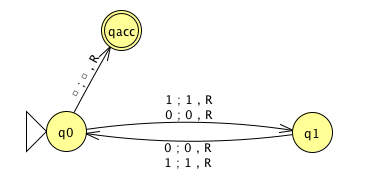
\includegraphics[width=2in]{../../resources/machines/Week8WarmupTM1.png} 

\columnbreak

$M_2$ 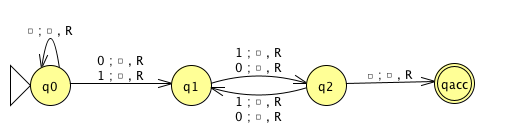
\includegraphics[width=2in]{../../resources/machines/Week8WarmupTM2.png}

\columnbreak

$M_3$ 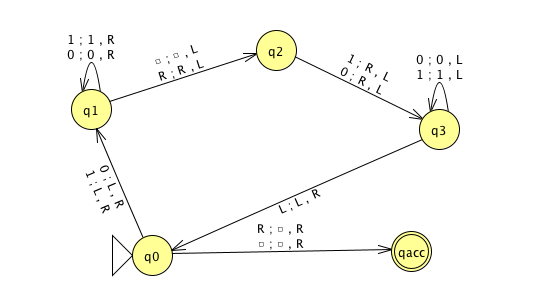
\includegraphics[width=2in]{../../resources/machines/Week8WarmupTM3.png}
\end{multicols}

Example strings in $A_{TM}$

\vfill

Example strings in  $E_{TM}$

\vfill

Example strings in  $EQ_{TM}$

\vfill

\newpage

{\bf  Theorem}: $A_{TM}$  is  Turing-recognizable.


{\bf  Strategy}:  To prove this theorem, we need  to  define  a Turing  machine  $R_{ATM}$ such that 
$L(R_{ATM}) = A_{TM}$.


Define $R_{ATM} =  $ ``

\vspace{150pt}


Proof of correctness: 


\vfill
\vfill

We will show that $A_{TM}$ is undecidable.   {\it First, let's explore what that means.}

\newpage

A {\bf Turing-recognizable} language is a set of strings that 
is the language recognized by some Turing machine. We also 
say that such languages are recognizable.

A {\bf Turing-decidable} language is a set of strings that 
is the language recognized by some decider. We also 
say that such languages are decidable.

An {\bf unrecognizable} language is a language that is not Turing-recognizable.

An {\bf undecidable} language is a language that is not Turing-decidable.


{\bf  True} or {\bf False}: Any  undecidable language  is  also  unrecognizable.


{\bf  True} or {\bf False}: Any  unrecognizable language  is  also  undecidable.


To prove that a computational problem is {\bf decidable}, we find/ build a Turing 
machine that recognizes the language encoding the computational problem, and that 
is a decider.


How do we prove a specific problem is {\bf not decidable}?

How would we even find such a computational problem?


{\it Counting arguments for the existence of an undecidable language:}
\begin{itemize}
    \item The set of all Turing machines is countably infinite.
    \item Each Turing-recognizable language is associated with a Turing machine
    in a one-to-one relationship, so there can be no more Turing-recognizable
    languages than there are Turing machines. 
    \item Since there are infinitely many Turing-recognizable languages
    (think of the singleton sets), there are countably infinitely 
    many Turing-recognizable languages.
    \item Such the set of Turing-decidable languages is an infinite subset 
    of the set of Turing-recognizable languages, the set of 
    Turing-decidable languages is also countably infinite.
\end{itemize}

Since there are uncountably many languages (because $\mathcal{P}(\Sigma^*)$
is uncountable), there are uncountably many unrecognizable languages
and there are uncountably many undecidable languages.


Thus, there's at least one undecidable language!

\vfill

{\bf What's a specific example of a language that is unrecognizable or undecidable?}

To prove that a language is undecidable, we need to prove that there is no Turing machine that decides it.

{\bf Key idea}: proof by contradiction relying on self-referential disagreement.

 \vfill
\section*{Week10 wednesday}



Recall: For  $M$ a deterministic decider, its {\bf running time} is the function  $f: \mathbb{N} \to \mathbb{N}$
given  by
\[
f(n) =  \text{max number of  steps $M$ takes before halting, over all inputs  of length $n$}
\]
For each function $t(n)$, the {\bf time complexity class}  $TIME(t(n))$, is defined  by
\[
TIME( t(n)) = \{ L \mid \text{$L$ is decidable by  a Turing machine with running time in  $O(t(n))$} \}
\]
$P$ is the class of languages that  are decidable in polynomial time on 
a deterministic 1-tape  Turing  machine
\[
P  =  \bigcup_k TIME(n^k)
\]

Definition (Sipser  7.9): For $N$ a nodeterministic decider.  
The {\bf running time} of $N$ is the function $f: \mathbb{N} \to \mathbb{N}$ given  by
\[
f(n) =  \text{max number of  steps $N$ takes on  any branch before halting, over all inputs  of length $n$}
\]

Definition (Sipser 7.21): For each function $t(n)$, the {\bf nondeterministic time complexity class}  
$NTIME(t(n))$, is defined  by
\[
NTIME( t(n)) = \{ L \mid \text{$L$ is decidable by a nondeterministic Turing machine with running time in $O(t(n))$} \}
\]
\[
NP = \bigcup_k NTIME(n^k)
\]


{\bf True} or {\bf False}: $TIME(n^2) \subseteq NTIME(n^2)$

\vfill

{\bf True} or {\bf False}: $NTIME(n^2) \subseteq DTIME(n^2)$

\vfill


{\bf Every problem in NP is decidable with an exponential-time algorithm}

Nondeterministic approach: guess a possible solution, verify that it works.

Brute-force (worst-case exponential time) approach: iterate over all possible solutions, for each 
one, check if it works.


\newpage

{\bf Examples in $P$ }

{\it Can't use nondeterminism; Can use multiple tapes; Often need to be “more clever” than naïve / brute force approach}
\[
    PATH = \{\langle G,s,t\rangle \mid \textrm{$G$ is digraph with $n$ nodes there is path from s to t}\}
\]
Use breadth first search to show in $P$
\[
    RELPRIME = \{ \langle x,y\rangle \mid \textrm{$x$ and $y$ are relatively prime integers}\}
\]
Use Euclidean Algorithm to show in $P$
\[
    L(G) = \{w \mid \textrm{$w$ is generated by $G$}\} 
\]
(where $G$ is a context-free grammar). Use dynamic programming to show in $P$.

\vfill
{\bf Examples in $NP$}

{\it ``Verifiable" i.e. NP, Can be decided by a nondeterministic TM in polynomial time,
best known deterministic solution may be brute-force, 
solution can be verified by a deterministic TM in polynomial time.}

\begin{align*}
    HAMPATH &= \{\langle G,s,t \rangle \mid \textrm{$G$ is digraph with $n$ nodes, }\\
    & \qquad \textrm{there is path
from $s$ to $t$ that goes through every node exactly once}\}
\end{align*}
\[
    VERTEX-COVER = \{ \langle G,k\rangle \mid \textrm{$G$ is an undirected graph with $n$
nodes that has a $k$-node vertex cover}\}
\]
\[
    CLIQUE = \{ \langle G,k\rangle \mid \textrm{$G$ is an undirected graph with $n$ nodes that has a $k$-clique}\}
\]
\[
    SAT =\{ \langle X \rangle \mid \textrm{$X$ is a satisfiable Boolean formula with $n$ variables}\}
\]

\begin{center}
\begin{tabular}{c|c}
    {\bf Problems in $P$} & {\bf Problems in $NP$}\\
    \hline
    (Membership in any) regular language & Any problem in $P$ \\
    (Membership in any) context-free language &  \\
    $A_{DFA}$ & $SAT$\\
    $E_{DFA}$ & $CLIQUE$ \\
    $EQ_{DFA}$ & $VERTEX-COVER$ \\
    $PATH$ & $HAMPATH$ \\
    $RELPRIME$ &  $\ldots$ \\
$\ldots$ &\\
\end{tabular}
\end{center}

\newpage

Million-dollar question: Is $P = NP$?


One approach to trying to answer it is to look for {\it hardest} problems in $NP$ and 
then (1) if we can show that there are efficient algorithms for them, then we can get 
efficient algorithms for all problems in $NP$ so $P = NP$, or (2) these problems might 
be good candidates for showing that there are problems in $NP$ for which there 
are no efficient algorithms.


Definition (Sipser 7.29) Language  $A$ is {\bf polynomial-time mapping reducible} to language $B$, written $A \leq_P B$,
means there is a polynomial-time computable function $f: \Sigma^* \to \Sigma^*$  such that for every $x \in \Sigma^*$
\[
x \in A \qquad \text{iff} \qquad f(x) \in B.
\]
The  function $f$ is  called the  polynomial time reduction of $A$ to $B$.

{\bf  Theorem}  (Sipser 7.31):  If $A \leq_P B$ and $B  \in P$ then $A \in P$.

Proof: 

\vfill

Definition (Sipser 7.34; based in Stephen Cook and Leonid Levin's work in the 1970s): 
A language $B$ is {\bf  NP-complete} means (1) $B$ is in NP {\bf and}  (2) every language
$A$ in $NP$ is polynomial time reducible to $B$.

{\bf  Theorem}  (Sipser 7.35):  If $B$ is NP-complete and $B \in P$ then $P = NP$.

Proof: 

\vfill

\newpage

{\bf 3SAT}: A literal is a Boolean variable (e.g.  $x$) or a negated Boolean variable (e.g.  $\bar{x}$).  
A Boolean formula is a {\bf  3cnf-formula} if it is a Boolean formula in conjunctive normal form (a conjunction  
of  disjunctive clauses of literals) and each clause  has  three literals.
\[
3SAT  = \{  \langle  \phi \rangle \mid \text{$\phi$ is  a  satisfiable 3cnf-formula} \}
\]


Example strings  in $3SAT$


Example  strings not  in $3SAT$




{\bf Cook-Levin Theorem}: $3SAT$ is $NP$-complete.


{\it Are there other $NP$-complete problems?} To prove that $X$ is $NP$-complete
\begin{itemize}
\item {\it From scratch}: prove $X$ is in $NP$ and that all $NP$ problems are polynomial-time
reducible to $X$.
\item {\it Using reduction}: prove $X$ is in $NP$ and that a known-to-be $NP$-complete problem 
is polynomial-time reducible to $X$.
\end{itemize}




{\bf CLIQUE}: A {\bf $k$-clique} in an undirected graph is a maximally connected subgraph with $k$  nodes.
\[
CLIQUE  = \{  \langle G, k \rangle \mid \text{$G$ is an  undirected graph with  a $k$-clique} \}
\]


Example strings  in $CLIQUE$


Example  strings not  in $CLIQUE$


Theorem (Sipser 7.32):
\[
3SAT  \leq_P CLIQUE
\]

Given a Boolean formula in conjunctive normal form with $k$ clauses and three literals per clause, we will 
map it to a graph so that the graph has a clique if the original formula is satisfiable and the 
graph does not have a clique if the original formula is not satisfiable.

The graph has $3k$ vertices (one for each literal in each clause) and an edge between all vertices except
\begin{itemize}
    \item vertices for two literals in the same clause
    \item vertices for literals that are negations of one another
\end{itemize}

Example: $(x \vee \bar{y} \vee {\bar z}) \wedge (\bar{x}  \vee y  \vee  z) \wedge (x \vee y  \vee z)$

\vfill

 \vfill
\section*{Week10 friday}


\begin{center}
    \begin{tabular}{|p{4in}|p{3.5in}|}
        \hline
        & \\
        {\bf Model of Computation} & {\bf Class of Languages}\\
        &\\
        \hline
        & \\
        {\bf Deterministic finite automata}:
        formal definition, how to design for a given language, 
        how to describe language of a machine?
        {\bf Nondeterministic finite automata}:
        formal definition, how to design for a given language, 
        how to describe language of a machine?
        {\bf Regular expressions}: formal definition, how to design for a given language, 
        how to describe language of expression?
        {\it Also}: converting between different models. &
        {\bf Class of regular languages}: what are the closure 
        properties of this class? which languages are not in the class?
        using {\bf pumping lemma} to prove nonregularity.\\
        & \\
        \hline
        & \\
        {\bf Push-down automata}:
        formal definition, how to design for a given language, 
        how to describe language of a machine?
        {\bf Context-free grammars}:
        formal definition, how to design for a given language, 
        how to describe language of a grammar? &
        {\bf Class of context-free languages}: what are the closure 
        properties of this class? which languages are not in the class?\\
        & \\
        \hline
        & \\
        Turing machines that always halt in polynomial time
        & $P$ \\
        & \\
        Nondeterministic Turing machines that always halt in polynomial time 
        & $NP$ \\
        & \\
        \hline
        & \\
        {\bf Deciders} (Turing machines that always halt): 
        formal definition, how to design for a given language, 
        how to describe language of a machine? &
        {\bf Class of decidable languages}: what are the closure properties 
        of this class? which languages are not in the class? using diagonalization
        and mapping reduction to show undecidability \\
        & \\
        \hline
        & \\
        {\bf Turing machines}
        formal definition, how to design for a given language, 
        how to describe language of a machine? &
        {\bf Class of recognizable languages}: what are the closure properties 
        of this class? which languages are not in the class? using closure
        and mapping reduction to show unrecognizability \\
        & \\
        \hline
    \end{tabular}
\end{center}

\newpage

{\bf Given a language, prove it is regular}

{\it Strategy 1}: construct DFA recognizing the language and prove it works.

{\it Strategy 2}: construct NFA recognizing the language and prove it works.

{\it Strategy 3}: construct regular expression recognizing the language and prove it works.

{\it ``Prove it works'' means \ldots}

\vspace{100pt}

{\bf Example}: $L  = \{ w \in \{0,1\}^* \mid \textrm{$w$ has odd number of $1$s or starts with $0$}\}$

Using NFA

\vfill

Using regular expressions

\vfill


\newpage

{\bf Example}: Select all and only the options that result in a true statement: ``To show 
a language $A$ is not regular, we can\ldots'' 

\begin{enumerate}
    \item[a.] Show $A$ is finite
    \item[b.] Show there is a CFG generating $A$
    \item[c.] Show $A$ has no pumping length
    \item[d.] Show $A$ is undecidable
\end{enumerate}

\newpage

{\bf Example}: What is the language generated by the CFG with rules
\begin{align*}
    S &\to aSb \mid bY \mid Ya \\
    Y &\to bY \mid Ya \mid \varepsilon 
\end{align*}

\newpage

{\bf Example}: Prove that the language 
$T = \{ \langle M \rangle \mid \textrm{$M$ is a Turing machine and $L(M)$ is infinite}\}$ 
is undecidable.

\newpage

{\bf Example}: Prove that the class of decidable languages is closed under concatenation.
 \vfill
\end{document}